% %%%%%%%%%%%%%%%%%%%%%%%%%%%%%%%%%%%%%%%%%%%%%%%%%%%%%%%%%%%%%%%%%%%%%
% %% Microarchitecture %%
% Introduction
% %%%%%%%%%%%%%%%%%%%%%%%%%%%%%%%%%%%%%%%%%%%%%%%%%%%%%%%%%%%%%%%%%%%%%

\section{Evaluation}
\label{sec:arch:eval}

TODO intro

% %%%%%%%%%%%%%%%%%%%%%%%%%%%%%%%%%%%%%%%%%%%%%%%%%%%%%%%%%%%%%%%%%%%%%
\subsection{Methodology for RTL Simulations}

The starting point is a CVA6~\cite{Zaruba2019_CVA6} RISC-V core with HPDcache~\cite{Fuguet2023_HPDcache} as an L1 data-cache with size 32~KiB ($S=128$, $W=4$, $l=8$ elements).
This serves as our baseline for performance comparison which we refer to as the \acrfull{gc}.
Next we evaluate a \gls{redC} which we derived from the HPDcache and configured to have two regions: a generic region with 16~KiB, and a \gls{reduction} region with 16~KiB whose behavior is the same as the \acrshort{drc} region of \acrlong{spdc}.
We refer to this design as \acrshort{redc}.
Finally, we evaluate \acrfull{spdc} with a reference configuration of: \acrshort{grc} = 8~KiB, \acrshort{drc} = 16~KiB, \acrshort{srt} = 8~KiB, which corresponds to the 25\%/50\%/25\% configuration selected in Chapter~\ref{cha:spdc}.
The configurations are summarized in Table~\ref{tab:arch:region_configs}.
All our simulations are performed using Siemens Questasim\texttrademark~2023.3 and the memory accesses beyond the L1 incur a fixed latency of 64 clock cycles.
We do not aim to evaluate a full system in this work, as our goal is to identify performance behavior using real matrices.
Thus, we use a single-core, single-cache-level environment.
The CVA6 core is not designed for high performance and can process at most one instruction per cycle.
We will discuss later how this limitation affects cache performance. \note{CHECK THIS AT THE END}
The fixed memory latency of 64 cycles is not realistic but provides a reasonable approximation of other memory levels' latencies and helps stabilize results for clearer interpretation.

% int64_t

% the hw constraint of the region sizes (could be fixed)

\begin{table}[htbp]
    \caption{Region Sizing of the Cache Configurations}
    \label{tab:arch:region_configs}
    \centering
    \begin{tblr}{
            width = {0.75\linewidth},
            colspec = {X[3cm,c] *{6}{X[c]}}, % rowspec
            rows = {m, font=\small},
            colsep = {1pt},
            row{1-Z} = {rowsep=2pt, black!2},
            column{2,4,6} = {r, rightsep=2pt},
            column{3,5,7} = {l, leftsep=2pt},
            row{1} = {c, font=\bfseries\small, black!5},
            cell{1}{2,4,6} = {c=2}{},
            hspan = {minimal},
            % hlines, vlines,
            % rulesep = {-1pt},
            hline{1,Z} = {2pt}, % Z for last
            hline{2} = {1pt},
            vline{2} = {1-Z}{0.5pt},
        }
        %
        Configurations & \acrshort{grc} & & \acrshort{drc} & & \acrshort{srt} & \\
        %
        \acrshort{gc}   & 100\% & ($S = 128$) & 0\%  & ($S = 0$)  & 0\%  & ($S = 0$)  \\
        \acrshort{redc} & 50\%  & ($S = 64$)  & 50\% & ($S = 64$) & 0\%  & ($S = 0$)  \\
        \acrshort{spdc} & 25\%  & ($S = 32$)  & 50\% & ($S = 64$) & 25\% & ($S = 32$)
    \end{tblr}
\end{table}

% %%%%%%%%%%%%%%%%%%%%%%%%%%%%%%%%%%%%%%%%%%%%%%%%%%%%%%%%%%%%%%%%%%%%%
\subsection{Sparse Formats Used for thr RTL Simulations}

By default, matrices are stored in \acrshort{csc} sparse format, and we use this format for most of our simulations.
However, in our evaluation, we try simulating \acrshort{spdc} with a specific format tailored for \acrshort{banded} matrices.
As shown in Figure~\ref{fig:arch:BaCSC}, compared to a \acrshort{csc}, we added extra information in the $ptr$ table to identify the beginning and end of the \gls{band}.
Indeed, three pointers instead of one are now needed per column, as shown with the example of column 2 in \textit{yellow}.
The column is split in one in-\gls{band} (IB) region in the middle and two out-of-\gls{band} (OB) regions around.
The $ptr$ table size thus becomes $3 \times M + 1$.
With this format, we can avoid the computational cost of identifying in which region non-zero elements are, while traversing the matrix, with the drawback of having to preprocess it.

\begin{figure}[htbp]
    \centering
    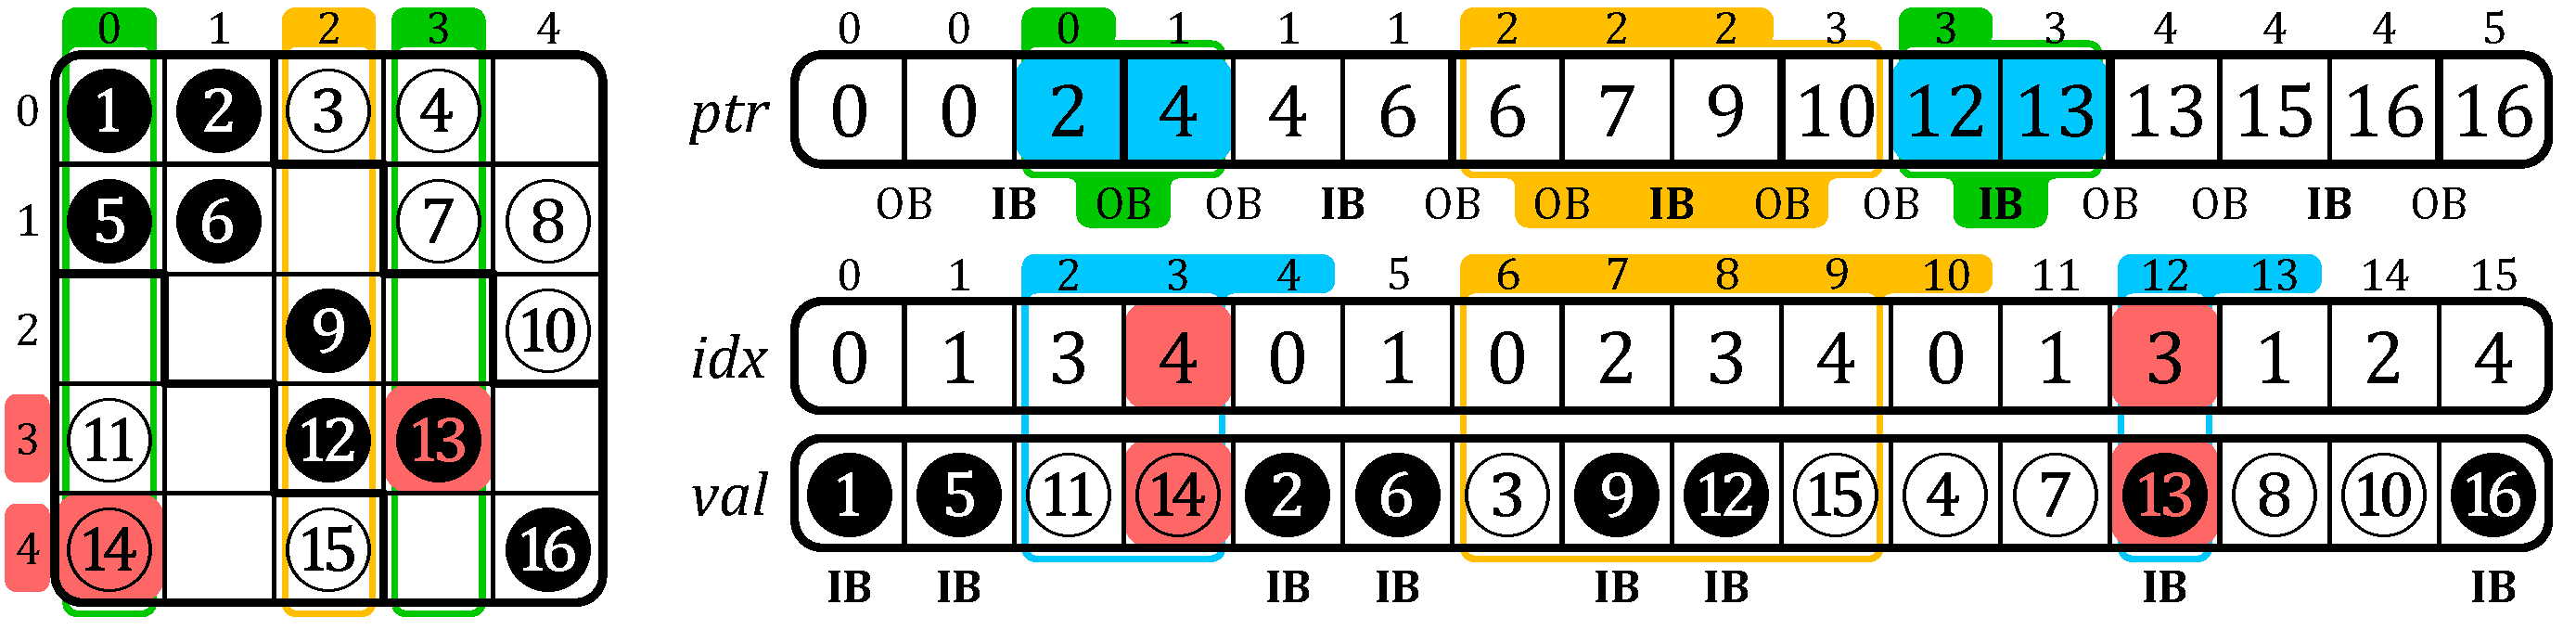
\includegraphics[width=\linewidth]{Chapter_MicroArch/Figures/PDF/SpFormats_BaCSC.pdf}
    \caption{Example of a Sparse Matrix in \acrshort{bacsc} Format}
    \label{fig:arch:BaCSC}
\end{figure}

\begin{highlight}{Conclusion}{Red}
    ..
\end{highlight}

% %%%%%%%%%%%%%%%%%%%%%%%%%%%%%%%%%%%%%%%%%%%%%%%%%%%%%%%%%%%%%%%%%%%%%
\subsection{Software Implementation of Outer-Product SpMV Kernel}

The code running on the CVA6 is written in generic C, compiled with \textit{gcc} 11.2.0 and -O3 optimization.
The \acrshort{red}-related instructions used in the \acrshort{op} \acrshort{spmv} kernel are manually inserted using \textit{asm} directives, as illustrated in Source Code~\ref{src:arch:op_spmv}.

\sourcecode{Chapter_MicroArch/Code/op_spmv.c}{C Code for the \acrshort{op} \acrshort{spmv} with \acrshort{red} Operations}{src:arch:op_spmv}{htbp}

The code shown is for \acrshort{spdc}.
Variants for other designs differ as follows: \acrshort{redc} omits region selection (line~15) and invokes \acrshort{reg} once before the loops with \acrshort{ibr} as the argument; \acrshort{gc} requires no \acrshort{reg} instruction and replaces \acrshort{red} with standard accumulation: $c[idx] \acc val$.

For \acrshort{spdc}, it is necessary to know the target region for each \acrshort{red} instruction based on the size of the \gls{band} (line~15).
The half-\gls{band} width $w_\mathit{hB}$ is derived from Chapter~\ref{cha:theory} (Equation~\ref{eq:theory:in_band_cond}) to ensure the in-\gls{band} region fits within the \acrshort{drc} independent of matrix structure.
In our reference configuration ($s_C(\mathit{DRC}) = 2048$, $l = 8$), $w_\mathit{hB} = 1021$.
Region selection follows Equation~\ref{eq:arch:reg_select} via an inline function, avoiding conditional branches within the inner-loop.

\begin{equation}
    \label{eq:arch:reg_select}
    \forall (i,j) \in \ldb 0, M-1 \rdb \times \ldb 0, N-1 \rdb, \; \mathit{region} = \left\{
    \begin{tabular}{ll}
        \acrshort{ibr} & if \; $|i-j| < w_\mathit{hB}$ \\
        \acrshort{obr} & else
    \end{tabular} \right.
\end{equation}

On-the-fly region computation introduces overhead in the critical inner-loop.
To mitigate this, we propose an alternative implementation (Source Code~\ref{src:arch:op_spmv_bacsc}) that precomputes regions and stores them using the \acrshort{bacsc} format.
Each column iteration begins with lookups in the outer-loop (line~5) to retrieve pointers for three sections: top out-of-\gls{band} (\textit{OB1}), in-\gls{band} (\textit{IB}), and bottom out-of-\gls{band} (\textit{OB2}).
The column is then processed through three separate inner-loops (lines~13, 21, 29) without region computation overhead.

\sourcecode{Chapter_MicroArch/Code/op_spmv_bacsc.c}{Optimized C Code for the \acrshort{op} \acrshort{spmv} when Using \acrshort{bacsc}}{src:arch:op_spmv_bacsc}{htbp}

Each approach trades off one limitation for another.
\acrshort{spdc}(\acrshort{csc}) uses simple \acrshort{csc} format with minimal preprocessing and low memory overhead, but incurs additional inner-loop instructions and thus latency per iteration.
\acrshort{spdc}(\acrshort{bacsc}) reduces instructions and latency at the cost of matrix preprocessing into \acrshort{bacsc} format and increased memory footprint.
Both variants are evaluated in the results section.

These software approaches avoid hardware modifications, providing flexibility.
However, hardware-computed regions with \acrshort{csc} format would eliminate the noted drawbacks.
A detailed breakdown of each design's instruction characteristics:
\begin{itemize}
    \item \acrshort{gc}: 10 inner-loop instructions; 3 instructions per \acrshort{red} with critical load dependency.
    \item \acrshort{redc}: 8 inner-loop instructions; 1 ``fire-and-forget'' \acrshort{red} instruction; 1 \acrshort{reg} setup per entire computation.
    \item \acrshort{spdc}(\acrshort{csc}): 14 inner-loop instructions; 1 ``fire-and-forget'' \acrshort{red} instruction; region computation within inner-loop.
    \item \acrshort{spdc}(\acrshort{bacsc}): 8 inner-loop instructions; 1 ``fire-and-forget'' \acrshort{red} instruction; outer-loop overhead.
\end{itemize}

To prevent software from limiting performance, we unroll inner-loops by a factor of 8 (not shown in Source Codes~\ref{src:arch:op_spmv} and~\ref{src:arch:op_spmv_bacsc}).
Each unrolled iteration executes 8 logical iterations with optimized instruction scheduling.
With cache-line size $l = 8$, this unrolling hides read-\gls{miss} latency through \glspl{hit} on consecutive addresses.
``Random'' \gls{reduction} accesses do not benefit from this latency hiding.
Consequently, \acrshort{gc} experiences potential latency from both \glspl{reduction} reads and writes, while \acrshort{redc} and \acrshort{spdc} benefit from ``fire-and-forget'' semantics and consecutive \gls{reduction} scheduling.

\acrshort{spdc}(\acrshort{csc}) is constrained to 4$\times$ unrolling due to register pressure on our platform.
This limitation, addressable with a higher-register CPU, demonstrates another advantage of hardware based region computation.

\begin{highlight}{Conclusion}{Red}
    ..
\end{highlight}

% %%%%%%%%%%%%%%%%%%%%%%%%%%%%%%%%%%%%%%%%%%%%%%%%%%%%%%%%%%%%%%%%%%%%%
\subsection{Matrix Selection for the RTL Evaluation}

We have selected an extended set of 62 square matrices from the SuiteSparse Matrix Collection~\cite{Kolodziej2019_SuiteSparse} which includes virtually all the matrices used by recent hardware accelerators~\cite{Zhang2021_Gamma, Xie2021_SpaceA, Zhang2022_ASA, Srikanth2021_SortCache, Pal2018_OuterSPACE}.
We verified that this set is diverse containing \gls{banded} and non-\gls{banded} sparse matrices with various sizes ($M \in [1.2\times10^{2}, 2.0\times10^{6}]$), numbers of non-zero elements ($nnz \in [2.2\times10^{3}, 1.4\times10^{7}]$) and a wide range of densities ($d \in [1.4\times10^{-6}, 7.8\times10^{-1}]$).

Based on our experimental results presented in the following section, we categorize these matrices into two groups according to their performance characteristics.
To facilitate this classification, we introduce a new metric, $d_\mathit{cd}$, defined as the average density of cache-line-sized clusters within matrix columns.
Specifically, for a cache with line size $l$, this metric quantifies the average density of non-empty cache-lines (or vertical-stripes as referenced in Chapter~\ref{cha:theory}), ranging between $\frac{1}{l}$ and 1.

%fig?

% When this metric is low ($d_\mathit{cd} \ll \frac{1}{l}$) the DRC is less effective and the problem tends to be memory-bound.
% When this metric is high ($d_\mathit{cd} \gg \frac{1}{l}$) there is significant spatial reuse in the cache and the problem tends to become compute-bound.

This metric provides a fine grain view of matrix density, which aligns more closely with cache characteristics.
When $d_\mathit{cd}$ approaches $\frac{1}{l}$ for a given matrix, it indicates that most non-zero elements are separated by at least $l$ zeros.
Consequently, the cache-lines are often nearly empty, which may render the line-wise \acrshort{drc} of a \acrshort{redc} inefficient, while the element-wise \acrshort{srt} of \acrshort{spdc} becomes more beneficial.
Conversely, as $d_\mathit{cd}$ increases, the non-zero elements of the matrix cluster more closely, enhancing the efficiency of the \acrshort{drc}.

In our experiments with $l = 8$, we establish two groups of matrices based on a $d_\mathit{cd}$ threshold of 20\%.
This threshold corresponds to a range of one to two non-zero elements per eight.
Although there is no definitive threshold, performance can vary significantly depending on the hardware environment.
In our scenario, using a simple scalar core, we can clearly distinguish matrices with highly isolated non-zero elements, thus setting the threshold at fewer than two elements per cache line.
A complete discussion on this follows in the next section.

According to this threshold, we categorize 21 matrices in group~1 ($d_\mathit{cd} \leqslant 20\%$) and 41 in group~2 ($d_\mathit{cd} > 20\%$).
We have selected 13 well-known matrices from both groups that are frequently used for performance evaluation, as illustrated in Table~\ref{tab:arch:matrices}.
The selected matrices represent a range of overall matrix densities ($d$) and $d_\mathit{cd}$ values, as depicted by the \textit{red} and \textit{purple} points in the scatter plot in Figure~\ref{fig:arch:matrices}.
In the following evaluation, we report the performance results of the 13 matrices from group~1 and~2, the geometric means for both groups on all matrices, and the overall geometric mean for the full set of 62 matrices.

\begin{table}[htbp]
    \centering
    \caption{Characteristics of Selected Group~1 and~2 Matrices}
    \label{tab:arch:matrices}
    \begin{tblr}{
            width = {0.8\linewidth},
            colspec = {X[c] X[c,2] *{4}{X[c]}}, % rowspec
            rows = {m, font=\small},
            colsep = {1pt},
            row{1-Z} = {rowsep=2pt, black!2},
            row{1} = {c, font=\bfseries\small, black!5},
            row{2,9} = {c, font=\bfseries\small},
            hspan = {minimal},
            % hlines, vlines,
            % rulesep = {-1pt},
            hline{1,Z} = {2pt}, % Z for last
            hline{2,3,9,10} = {1pt},
        }
        %
        ID & Matrix & M & nnz & Density & d\textsubscript{cd} \\
        Group 1 \\
        11 & poisson3Da    & 13.5~k & 352~k  & 1.93 e-3 & 14\% \\
        12 & cit-HepTh     & 27.8~k & 353~k  & 4.57 e-4 & 13\% \\
        13 & soc-Epinions1 & 75.8~k & 508~k  & 8.84 e-5 & 16\% \\
        14 & sme3Db        & 29.1~k & 2.08~M & 2.46 e-3 & 15\% \\
        15 & Stanford      & 282~k  & 2.31~M & 2.91 e-5 & 12\% \\
        16 & web-Google    & 916~k  & 5.11~M & 6.08 e-6 & 13\% \\
        Group 2 \\
        21 & msc10848 & 10.8~k & 1.23~M & 1.05 e-2 & 73\% \\
        22 & opt1     & 15.4~k & 1.93~M & 8.09 e-3 & 86\% \\
        23 & bcsstk32 & 44.6~k & 2.01~M & 1.01 e-3 & 75\% \\
        24 & xenon2   & 15.7~k & 2.87~M & 1.56 e-4 & 40\% \\
        25 & consph   & 83.3~k & 6.01~M & 8.66 e-4 & 57\% \\
        26 & x104     & 108~k  & 10.0~M & 8.66 e-4 & 78\% \\
        27 & pwtk     & 218~k  & 11.6~M & 2.45 e-4 & 75\%
        %
    \end{tblr}
\end{table}

\begin{figure}[htbp]
    \centering
    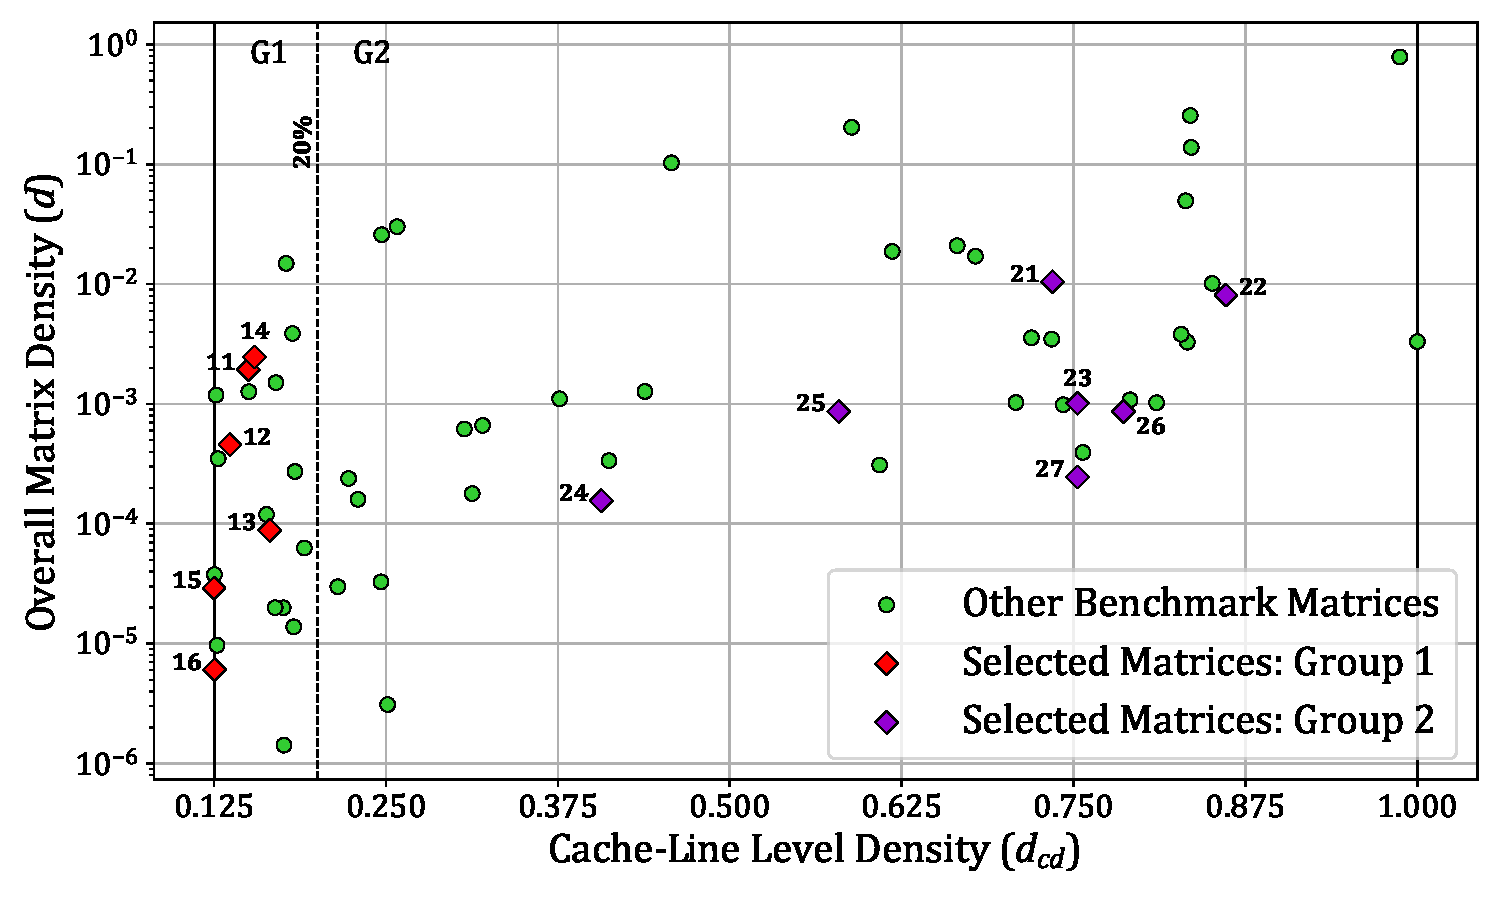
\includegraphics[width=\linewidth]{Chapter_MicroArch/Figures/PDF/BenchmarkMatricesDcdRep.pdf}
    \caption{Benchmark Matrices: $d_\mathit{cd}$ vs $nnz/Column$}
    \label{fig:arch:matrices}
\end{figure}

\begin{highlight}{Conclusion}{Red}
    The benchmark matrices are divided into two groups depending on $d_\mathit{cd}$, their average cache-line-sized clusters density.
\end{highlight}

% %%%%%%%%%%%%%%%%%%%%%%%%%%%%%%%%%%%%%%%%%%%%%%%%%%%%%%%%%%%%%%%%%%%%%
\subsection{Results Analysis}

% %%%%%%%%%%%%%%%%%%%%%%%%%%%%%%%%%%%%%%%%%%%%%%%%%%%%%%%%%%%%%%%%%%%%%
\subsubsection{Memory Traffic}

For all the benchmark matrices, we simulated the SystemVerilog model executing the full \algo{OP} SpMV and initially measured the memory traffic for the output vector as shown in Figure~\ref{fig:arch:outmemtraffbar} for \textit{RedC}, OBaMMA with BaCSC and OBaMMA with CSC.
These results are expressed as a ratio compared to the memory traffic for \textit{GC}.
OBaMMA achieves a remarkable $3.9\times$ reduction in memory traffic which is over $2.7\times$ lower compared to \textit{RedC}. 
OBaMMA performs well for the matrices in both groups.
Since \textit{GC} performs better for group~2, the relative benefit of OBaMMA is smaller but still significant.
With OBaMMA, the data in the DRC is dense and stays in the cache from column to column enabling the rotating pattern of Section~\ref{sec:theory} to occur.
Outside of the DRC, the opportunities for reuse are limited and the element-wise, fully-associative storage makes best use of the memory bandwidth by avoiding the transfer of mostly empty cache-lines.

Note that for the group~1 matrices, the \textit{RedC} traffic is higher than for \textit{GC}.
Indeed, when the cache-lines are always sparsely used, the cache is ineffective, both for \textit{GC} and \textit{RedC}.
In our configuration, the size of \textit{GC} is 2$\times$ larger than the DRC region in the \textit{RedC}, which explains the better performance.
For the group~2 matrices, the cache becomes effective, as the cache-lines frequently hit, and it becomes possible to take advantage of the in-memory accumulation provided by \textit{RedC}.

So far, we focused on output memory traffic.
To perform an \algo{OP} SpMV, the input matrix and input vector are read once in a linear fashion~\cite{Isaac2024_SoA}.
Figure~\ref{fig:arch:inoutmetraff} shows the distribution of the total memory traffic including inputs and the output vector.
We note the stark difference in behavior between the group~1 and group~2 matrices.
For group~1, with traditional caches, the output traffic is high because near empty cache-lines are frequently transferred back and forth to main memory and, this is one of the reasons that \algo{OP} algorithms are less used, despite having theoretically better performance~\cite{Mukkara2019_PHI, Isaac2024_SoA}.
For these matrices, OBaMMA greatly reduces the output traffic providing a $2.7\times$ reduction in overall traffic.
For the group~2 matrices, OBaMMA still provides a $17\%$ reduction in overall traffic, although these matrices already perform well with traditional caches.
For \textit{GC}, \textit{RedC} and OBaMMA with CSC, the volume of input traffic is constant. 
With OBaMMA, the preprocessing adds a small input traffic overhead ($< 10\%$).

\begin{figure}[htbp]
    \centering
    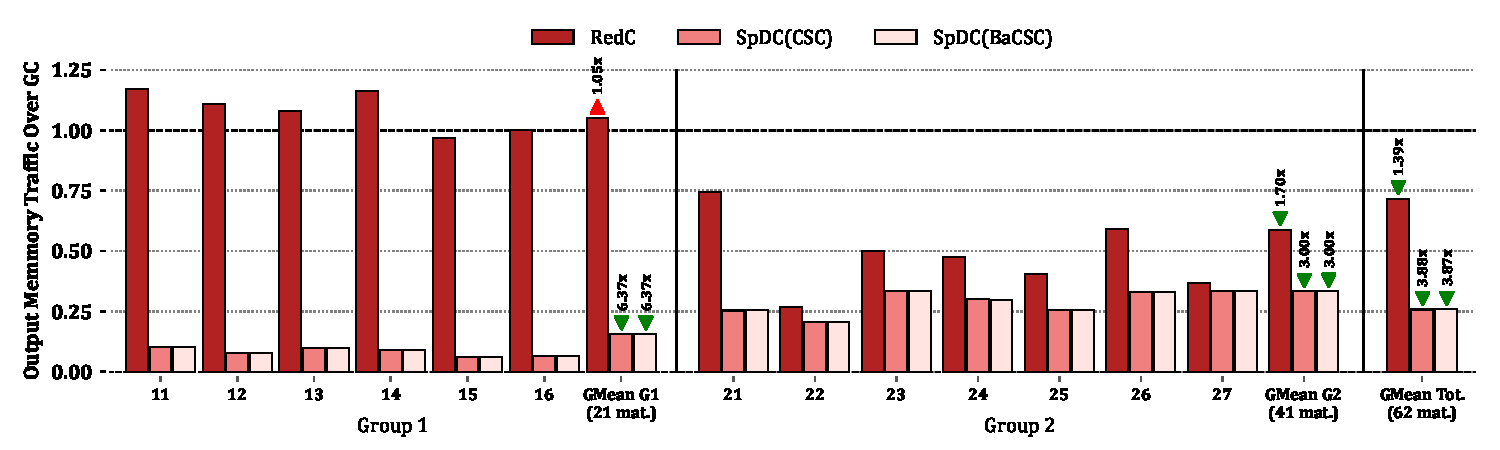
\includegraphics[width=\linewidth]{Chapter_MicroArch/Figures/PDF/OutMemTrafficFromRTL.pdf}
    \caption{Output Memory Traffic Normalized over \acrshort{gc}, from \acrshort{rtl} Simulations}
    \label{fig:arch:outmemtraffbar}
    % \label{fig:arch:outMT}
\end{figure}

\begin{figure}[htbp]
    \centering
    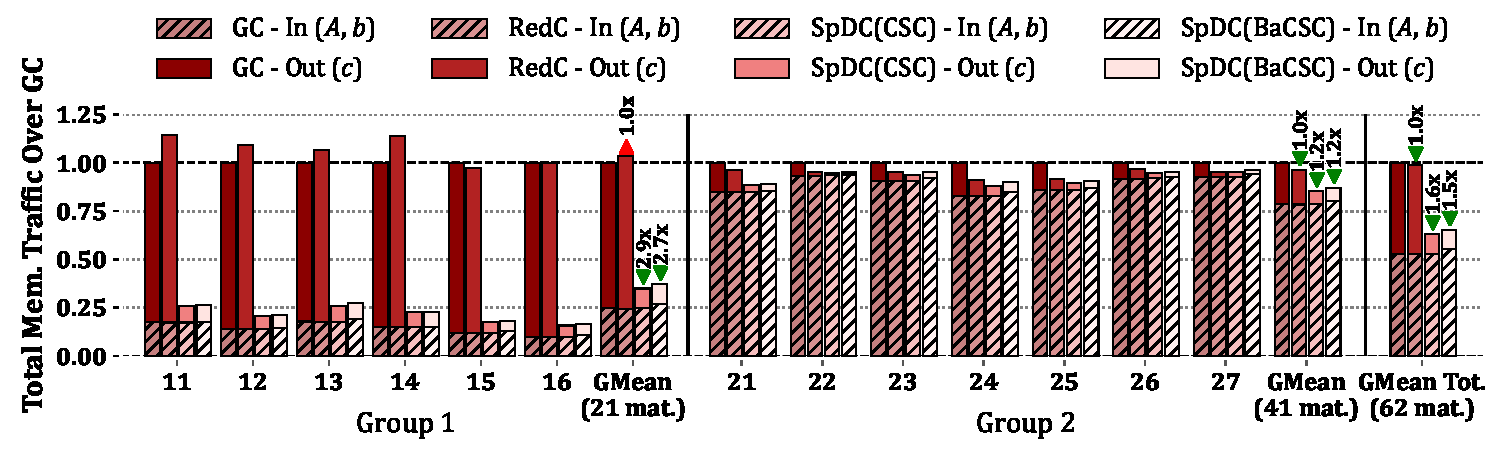
\includegraphics[width=\linewidth]{Chapter_MicroArch/Figures/PDF/TotMemTrafficFromRTL.pdf}
    \caption{Total Memory Traffic on Input Matrix $A$, Input Vector $b$ and Output Vector $c$, Normalized over \acrshort{gc}, from \acrshort{rtl} Simulations}
    \label{fig:arch:inoutmetraff}
    % \label{fig:arch:totMT}
\end{figure}

% %%%%%%%%%%%%%%%%%%%%%%%%%%%%%%%%%%%%%%%%%%%%%%%%%%%%%%%%%%%%%%%%%%%%%
\subsubsection{Latencies}

Our focus now shifts to the total compute time, and we recall that all main memory reads incur a fixed 64 cycle latency.
Figure~\ref{fig:arch:speedup} shows the speedup compared to execution on \textit{GC}.
For the group~1 matrices, we first note that \textit{RedC} achieves some speedup $(1.09\times$) which can be explained as the RED operation is ``fire-and-forget'' for the processor, however, they can quickly block in the cache if the \textit{accumulation table} (\textit{AccTab}) is busy processing the previous request.
In the group~1 matrices, because the cache-lines are sparse, there are frequently bursts of evictions making this effect dominant, thus the system is memory bound.
OBaMMA slightly outperforms \textit{RedC} because it can also issue ``fire-and-forget'' element-wise memory transactions which reduces the blocking.

For the group~2 matrices, particularly, with our single core RISC-V processor, the system becomes compute bound.
For OBaMMA with CSC, there is an overhead to calculate the region which results in some slow down ($-1.36\times$), however, with preprocessing, this overhead is removed and OBaMMA achieves the same latencies as \textit{GC}.

\begin{figure}[htbp]
    \centering
    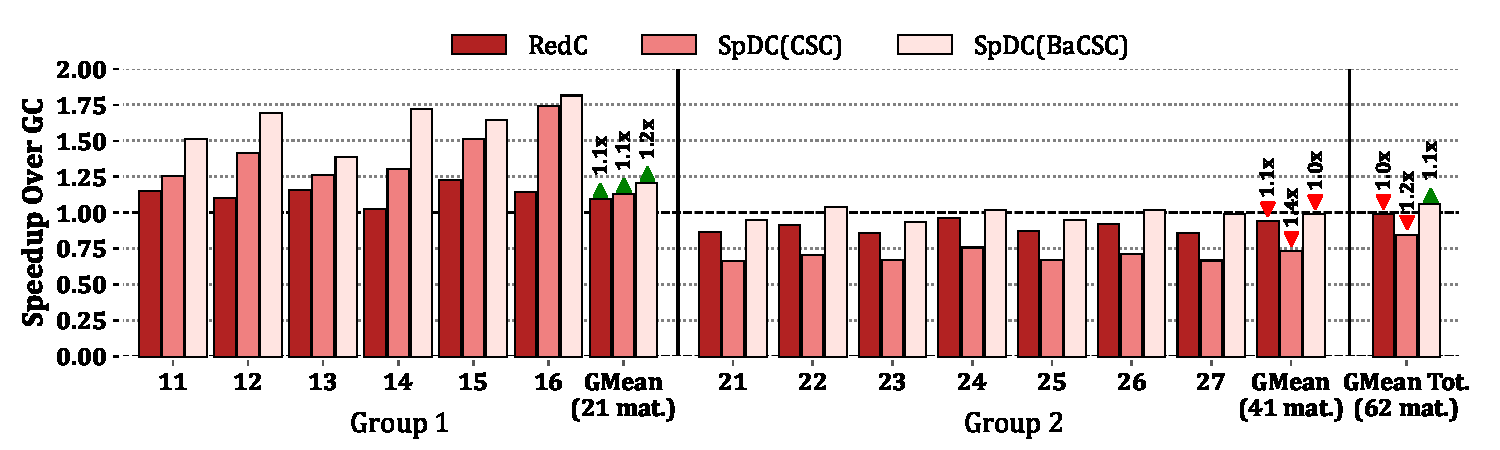
\includegraphics[width=\linewidth]{Chapter_MicroArch/Figures/PDF/Speedups.pdf}
    \caption{Speedup over \acrshort{gc}, from \acrshort{rtl} Simulations}
    \label{fig:arch:speedup}
\end{figure}

% %%%%%%%%%%%%%%%%%%%%%%%%%%%%%%%%%%%%%%%%%%%%%%%%%%%%%%%%%%%%%%%%%%%%%
\subsubsection{Discussion over the Two Performance Groups}

%discussion using slide

Two parameters characterize sparse matrices: (1) the $nnz/Column$ which is a coarse-grain measure of density and (2) the $d_\mathit{cd}$ which is a measure of the density at the granularity of a cache-line.
In Figure~\ref{fig:arch:allscatter}, the normalized memory traffic ($bytes/nnz$) for each of the matrices is shown for \textit{RedC} and OBaMMA.
With \textit{RedC}, the memory traffic is high for low values of $d_\mathit{cd}$ whereas for OBaMMA, the memory traffic is virtually independent of both density parameters.

\begin{figure}[htbp]
    \centering
    \begin{subfigure}{0.49\linewidth}
        \centering
        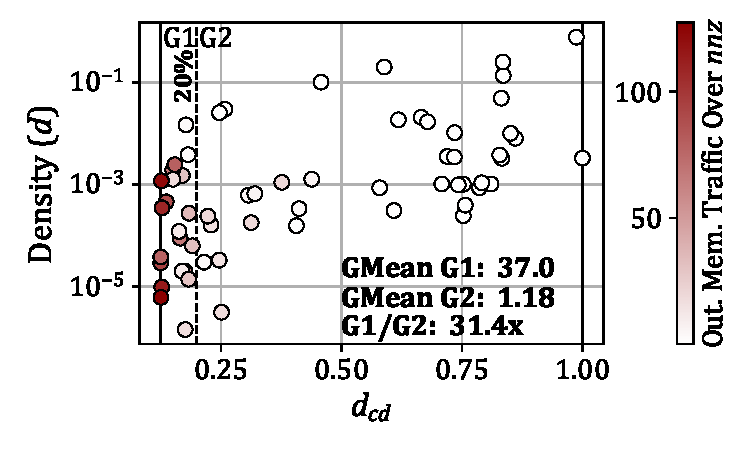
\includegraphics[width=\linewidth]{Chapter_MicroArch/Figures/PDF/MatricesDcdRep_WithMT_onRedC.pdf}
        \caption{\acrshort{redc} Output Memory Traffic over \acrshort{gc}}
        \label{fig:arch:perfOnMat:00}
    \end{subfigure}
    \hfill
    \begin{subfigure}{0.49\linewidth}
        \centering
        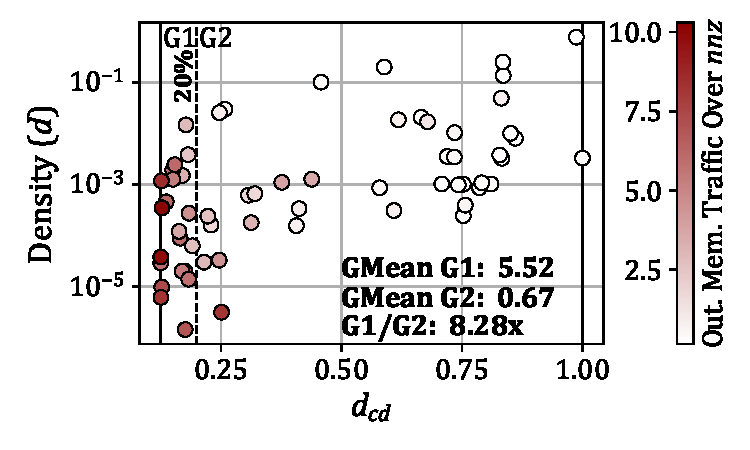
\includegraphics[width=\linewidth]{Chapter_MicroArch/Figures/PDF/MatricesDcdRep_WithMT_onSpDC.pdf}
        \caption{\acrshort{spdc} Output Memory Traffic over \acrshort{gc}}
        \label{fig:arch:perfOnMat:01}
    \end{subfigure}
    %
    \begin{subfigure}{0.49\linewidth}
        \centering
        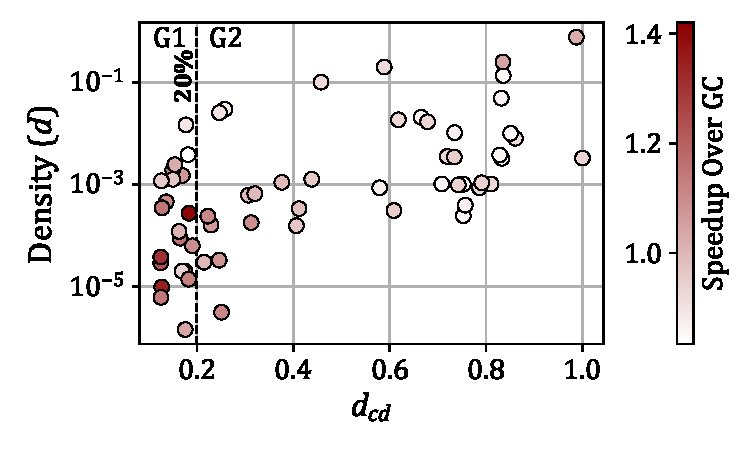
\includegraphics[width=\linewidth]{Chapter_MicroArch/Figures/PDF/MatricesDcdRep_WithSpeedUp_onRedC.pdf}
        \caption{\acrshort{redc} Speedup over \acrshort{gc}}
        \label{fig:arch:perfOnMat:10}
    \end{subfigure}
    \hfill
    \begin{subfigure}{0.49\linewidth}
        \centering
        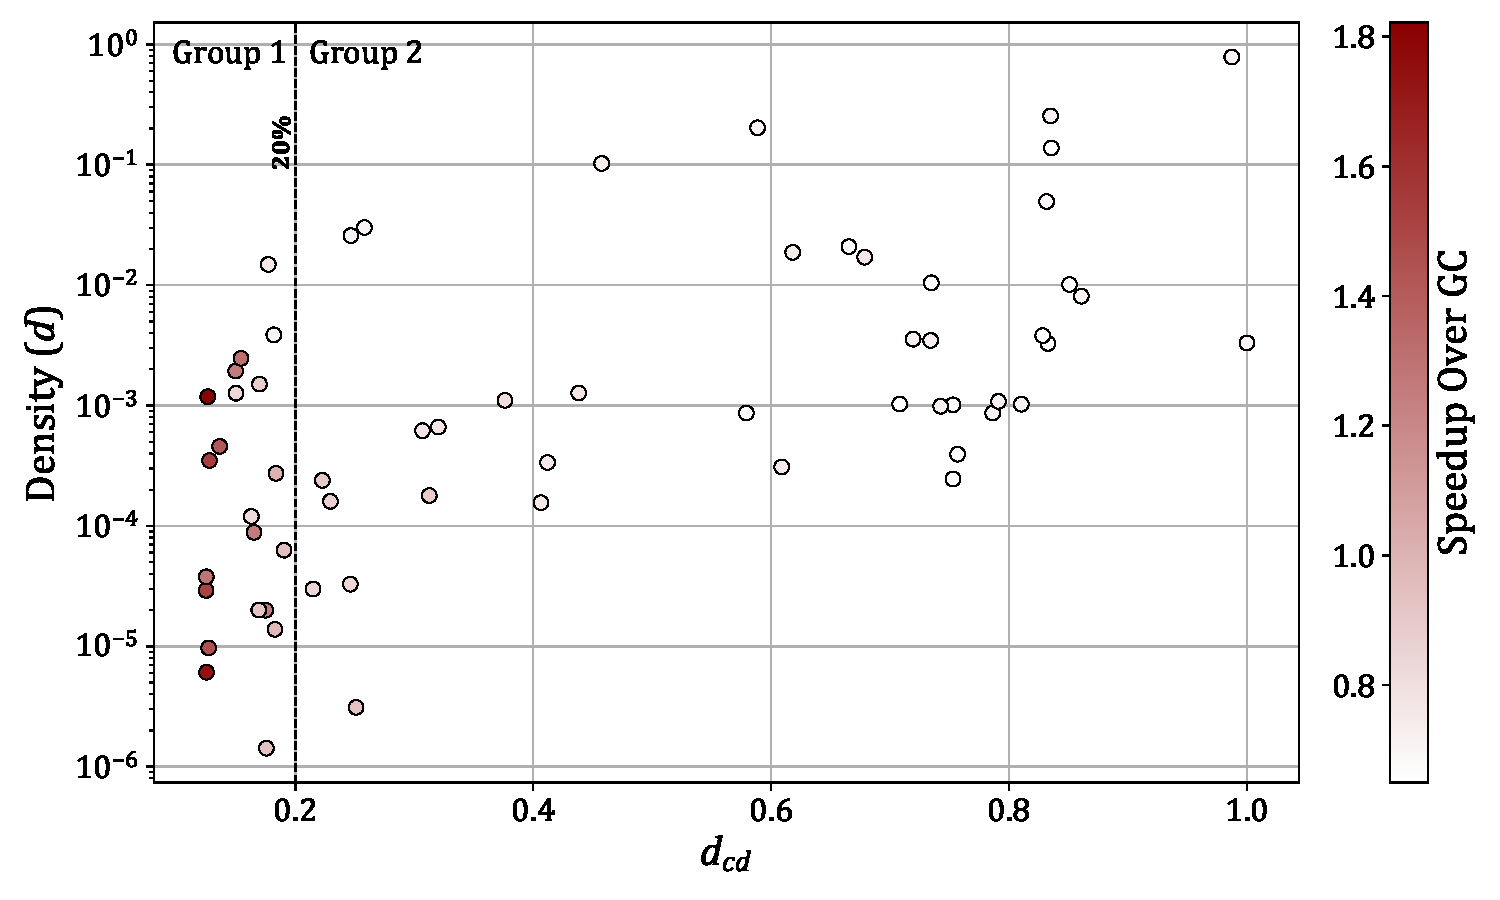
\includegraphics[width=\linewidth]{Chapter_MicroArch/Figures/PDF/MatricesDcdRep_WithSpeedUp_onSpDC.pdf}
        \caption{\acrshort{spdc} Speedup over \acrshort{gc}}
        \label{fig:arch:perfOnMat:11}
    \end{subfigure}
    \caption{Memory Traffic and Speedup Performance Visualized Across Benchmark Matrix Densities and $d_\mathit{cd}$}
    \label{fig:arch:perfOnMat}
\end{figure}

To summarize, the group~1 matrices are the ones that perform poorly with traditional caches, and for this group, OBaMMA achieves a $2.4\times$ reduction in memory traffic and a speedup of $1.21\times$.
In a processor with more compute resources (e.g. multicore) the pressure on the memory system would be greater and the majority of matrices would behave as the group~1 matrices.
Indeed, with OBaMMA, the memory traffic is insensitive to the characteristics of the matrices as shown in Figure~\ref{fig:arch:allscatter} which makes for predictable performance.

We previously discussed how the single-entry \textit{AccTab} was a performance bottleneck for \textit{RedC}. 
We investigate the impact of increasing the \textit{AccTab} entries from 1 to 8, presenting the speedup relative to \textit{GC} for selected group~1 and~2 matrices.

For the matrices in group~2, which are compute bound, increasing the \textit{AccTab} entries has no impact on runtime ($\leqslant 1\%$).
In the case of group~1 matrices, setting the \textit{AccTab} to 1, 2, 4, and 8 entries allows \textit{RedC} to achieve performance improvements of $1.16\times$, $1.36\times$, $1.60\times$, and $1.61\times$ respectively, compared to \textit{GC}, although this comes at the cost of increased area.
For OBaMMA, increasing the \textit{AccTab} has virtually no impact regardless of the matrices ($\leqslant 0.5\%$).
This is expected as there are rarely evictions from the DRC as it is sized to contain the \gls{band}.
OBaMMA's region based architecture thus reduces both total memory traffic and memory bursts.

% %%%%%%%%%%%%%%%%%%%%%%%%%%%%%%%%%%%%%%%%%%%%%%%%%%%%%%%%%%%%%%%%%%%%%
\subsubsection{Area Overhead}

Both HPDcache and OBaMMA systems were synthesized in GF22FDX technology using Synopsis DC\texttrademark.
The original area was $0.99~mm^2$ and the OBaMMA version was $1.3~mm^2$, an increase of $26\%$.
This shows that OBaMMA could reasonably be integrated into a processor, providing a large performance improvement ($3.9\times$ in memory traffic), with an area overhead that is much lower than predicted by Borkar's law~\cite{Borkar2007_AreaOverheads}.
% GC 991638,916 um2 / OBaMMA 1252208,92 um2 / 26%

% %%%%%%%%%%%%%%%%%%%%%%%%%%%%%%%%%%%%%%%%%%%%%%%%%%%%%%%%%%%%%%%%%%%%%
\subsection{Comparison with the Analytical Model}

To validate consistency between our models and implementations, we compare the normalized output memory traffic produced by three sources: the analytical model of Chapter~\ref{cha:theory}, the Python model of Chapter~\ref{cha:spdc}, and the \acrshort{rtl} implementation presented in this chapter.
For a fair comparison, the caches for \acrshort{redc} and \acrshort{spdc} are configured to 32~KiB total (see Table~\ref{tab:arch:region_configs}): 50\%/50\%/0\% for \acrshort{redc} and 25\%/50\%/25\% for \acrshort{spdc}.
The analytical model accepts global parameters and density distributions rather than concrete matrices, so we synthesize \gls{banded} matrices for the Python and \acrshort{rtl} simulations that match those parameters.
All synthetic matrices use $M = 10^{4}$, half-\gls{band} width $w_\mathit{hB} = 1021$, in-\gls{band} density $d_\mathit{IB} = 10^{-2}$, and out-of-\gls{band} density $d_\mathit{OB}$ varying from $10^{-7}$ to $10^{-2}$.
Note that at $d_\mathit{OB} \simeq 8\times10^{-3}$, approximately one non-zero element exists per column in the out-of-\gls{band} region, whereas at $d_\mathit{OB} \simeq 8\times10^{-7}$, approximately one non-zero element exists in the entire out-of-\gls{band} region, resulting in a nearly \gls{PBanded} matrix.

\begin{figure}[htbp]
    \centering
    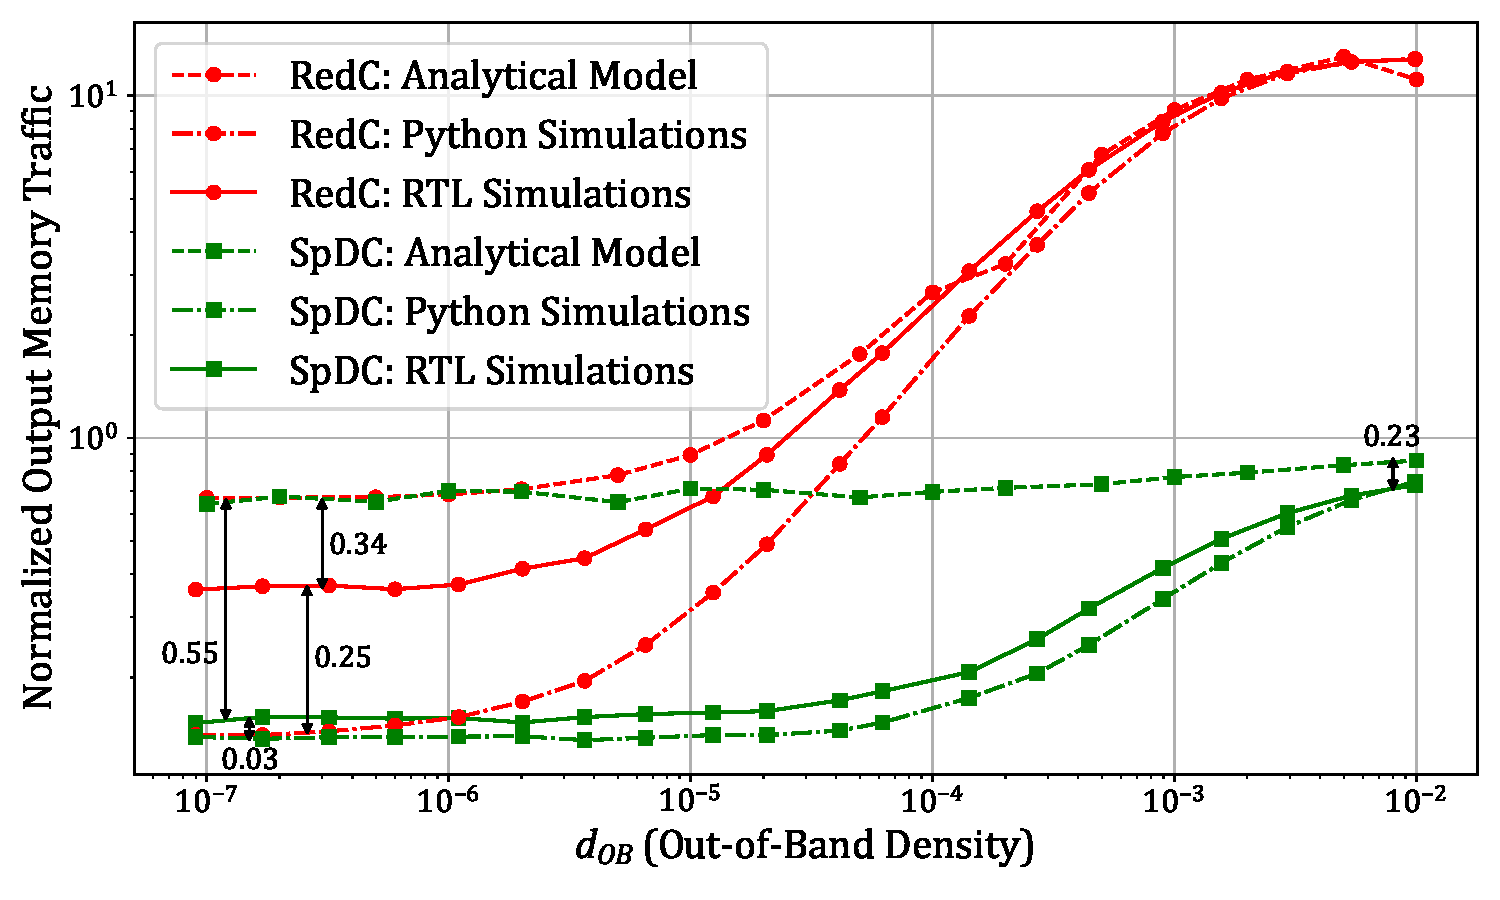
\includegraphics[width=\linewidth]{Chapter_MicroArch/Figures/PDF/graph11_25.12.02.pdf}
    \caption{Normalized Output Memory Traffic Depending on the Out-of-Band Density for the \acrshort{redc} and \acrshort{spdc} Configurations, Through Different Simulation Models}
    \label{fig:arch:graph11}
\end{figure}

Figure~\ref{fig:arch:graph11} shows the results: \acrshort{spdc} (\textit{green}) outperforms \acrshort{redc} (\textit{red}) in normalized output memory traffic ($\mathit{normMT}$).
Two observations are noteworthy.
First, the three approaches agree most closely when $d_\mathit{OB}$ is low.
Indeed, at $d_\mathit{OB} = 10^{-2}$ there is no measurable difference for \acrshort{redc}, while \acrshort{spdc} exhibits a 0.23 difference in $\mathit{normMT}$.
At the smallest $d_\mathit{OB}$ the discrepancies reach 0.58 element transferred in memory per \gls{reduction}.
Overall trends are preserved across models and deviations remain small.
Second, the analytical model consistently overestimates traffic, the Python model consistently underestimates it, and the \acrshort{rtl} results fall between the two.

\begin{highlight}{Conclusion}{Red}
    Across synthetic \gls{banded} matrices, all three simulation models demonstrate consistent memory traffic results, with only minor divergences as matrices approach the \gls{PBanded} regime.
\end{highlight}

% %%%%%%%%%%%%%%%%%%%%%%%%%%%%%%%%%%%%%%%%%%%%%%%%%%%%%%%%%%%%%%%%%%%%%
\subsection{Comparison with the Python Model}

To further validate our implementation over real, not necessarily \gls{banded}, matrices, we compare the \acrshort{rtl} results against the Python simulations from Chapter~\ref{cha:spdc}.
Table~\ref{tab:arch:results_python} presents the Python results for the \acrshort{rtl} cache configurations shown in Table~\ref{tab:arch:region_configs}.
We include the \acrshort{redc} 50\%/50\%/0\% configuration for comparison, though it is suboptimal according to the Python analysis.
Table~\ref{tab:arch:rtl_vs_python} reports \acrshort{rtl} results with geometric mean over the same 48 matrices used in Python simulations, comparing output and total memory traffic.

\begin{figure}[htbp]
    \centering
    \begin{minipage}[t]{0.49\linewidth}
        \centering
        \begin{table}[H]
            \caption{Results of Main Cache Configurations from Python Simulation}
            \label{tab:arch:results_python}
            \centering
            \begin{tblr}{
                    width = {0.88\linewidth},
                    colspec = {X[1.7,c] X[0.5,c] X[0.8,c] *{3}{X[c]}}, % rowspec
                    rows = {m, font=\small},
                    colsep = {1pt},
                    column{1-3} = {colsep=0pt},
                    column{1} = {leftsep=1pt},
                    column{3} = {rightsep=1pt},
                    row{1-Z} = {rowsep=2pt, black!2},
                    row{1} = {c, font=\bfseries\small, black!5},
                    column{1} = {l},
                    row{2-4} = {c, black!5},
                    row{2-4} = {font=\itshape\small},
                    row{2-4} = {rowsep=0pt},
                    row{6,9,11,13} = {abovesep=0pt},
                    row{5,8,10,12} = {belowsep=0pt},
                    cell{2}{2} = {r=3}{c},
                    cell{2-4}{1} = {r},
                    cell{5,8,10,12}{1} = {r=2}{},
                    cell{5-13}{1} = {c=3}{},
                    cell{1}{1} = {r=2}{},
                    hspan = {minimal},
                    % hlines, vlines,
                    % rulesep = {-1pt},
                    hline{1,Z} = {2pt}, % Z for last
                    hline{5} = {1pt},
                    vline{4} = {1-Z}{0.5pt},
                }
                %
                GMeans (48 mat.) & & & \acrshort{gc} & \acrshort{redc} & \acrshort{spdc} \\
                %
                & \rotatebox[y=2pt]{90}{\glspl{set}} & \acrshort{grc}\; & 128 & 64 & 32 \\
                &                                    & \acrshort{drc}\; & \O  & 64 & 64 \\
                &                                    & \acrshort{srt}\; & \O  & \O & 32 \\
                %
                \textbf{Output Memory Traffic} (\% over GC)      & & & 100  & 103 & 24.5 \\
                                                                & & & \cst1.0 & \cst1.0 & \dwG4.1 \\
                \textbf{Ratio of RMWs in Memory Traffic} (\%)    & & & \O   & \O   & 40.5 \\
                \textbf{Total Memory Traffic} (\% over GC)       & & & 100  & 98.5 & 56.1 \\
                                                                & & & \cst1.0 & \cst1.0 & \dwG1.8 \\
                \textbf{Evicted Cache Line Utilization} (max: 8) & & & 3.60 & 3.41 & 7.21 \\
                                                                & & & \cst1.0 & \cst1.0 & \upG2.0 \\
                \textbf{Cache Memory Utilization} (\%)           & & & 36.4 & 43.8 & 75.2 \\
                                                                & & & \cst1.0 & \upG1.2 & \upG2.1 \\
                %
            \end{tblr}
        \end{table}
    \end{minipage}
    \hfill
    \begin{minipage}[t]{0.49\linewidth}
        \centering
        \begin{table}[H]
            \caption{\acrshort{rtl} Results Comparison with Python Simulations}
            \label{tab:arch:rtl_vs_python}
            \centering
            \begin{tblr}{
                    width = {0.88\linewidth},
                    colspec = {X[1.7,c] X[0.5,c] X[0.8,c] *{3}{X[c]}}, % rowspec
                    rows = {m, font=\small},
                    colsep = {1pt},
                    column{1-3} = {colsep=0pt},
                    column{1} = {leftsep=1pt},
                    column{3} = {rightsep=1pt},
                    row{1-Z} = {rowsep=2pt, black!2},
                    row{1} = {c, font=\bfseries\small, black!5},
                    column{1} = {l},
                    row{2-4} = {c, black!5},
                    row{2-4} = {font=\itshape\small},
                    row{2-4} = {rowsep=0pt},
                    row{6,8,10,12} = {abovesep=0pt},
                    row{5,7,9,11} = {belowsep=0pt},
                    cell{2}{2} = {r=3}{c},
                    cell{2-4}{1} = {r},
                    cell{5,7,9,11}{1} = {r=2}{},
                    cell{5-Z}{1} = {c=3}{},
                    cell{1}{1} = {r=2}{},
                    hspan = {minimal},
                    % hlines, vlines,
                    % rulesep = {-1pt},
                    hline{1,Z} = {2pt}, % Z for last
                    hline{5} = {1pt},
                    vline{4} = {1-Z}{0.5pt},
                }
                %
                GMeans (48 mat.) & & & \acrshort{gc} & \acrshort{redc} & \acrshort{spdc} \\
                %
                & \rotatebox[y=2pt]{90}{\glspl{set}} & \acrshort{grc}\; & 128 & 64 & 32 \\
                &                                    & \acrshort{drc}\; & \O  & 64 & 64 \\
                &                                    & \acrshort{srt}\; & \O  & \O & 32 \\
                %
                \textbf{Output Memory Traffic} (\% over GC) & & & 100  & 75.5 & 20.0 \\
                                                            & & & \cst1.0 & \dwG1.3 & \dwG5.0 \\
                $\rightarrow$ \textbf{RTL/Python} (\%)      & & & 116 & 85.0 & 94.6 \\
                                                            & & & \upR0.9 & \dwG1.2 & \dwG1.1 \\
                \textbf{Total Memory Traffic} (\% over GC)  & & & 100  & 99.3 & 54.7 \\
                                                            & & & \cst1.0 & \cst1.0 & \dwG1.8 \\
                $\rightarrow$ \textbf{RTL/Python} (\%)      & & & 75.5 & 76.1 & 73.6 \\
                                                            & & & \dwG1.3 & \dwG1.3 & \dwG1.4 \\
                %
            \end{tblr}
        \end{table}
    \end{minipage}
\end{figure}

The total memory traffic for \acrshort{redc} and \acrshort{spdc} relative to \acrshort{gc} is nearly equivalent across both simulations.
However, output memory traffic shows notable differences: \acrshort{rtl} achieves better traffic reduction than Python, 1.3$\times$ for \acrshort{redc} (vs. 1.0$\times$ in Python) and 5.0$\times$ for \acrshort{spdc} (vs. 4.1$\times$ in Python).
Comparing raw traffic values between \acrshort{rtl} and Python simulations across all configurations, we observe approximately 25\% lower total memory traffic in \acrshort{rtl}.
Output memory traffic varies by $\pm$15\%, with \acrshort{rtl} showing favorable results for both \acrshort{redc} and \acrshort{spdc}.

\begin{highlight}{Conclusion}{Red}
    Over a set of real application matrices, the \acrshort{rtl} implementation corroborates the Python simulations, exhibiting slightly improved memory traffic performance.
\end{highlight}